\section{The Need for Dynamic Load Balancing Policies}
\label{sec:the-need-for-dynamic-load-balancing-policies}

% why is the performance lower for smaller caches?
Despite the memory savings, our results suggest that dynamic load balancing
policies could save even more memory.  Figure~\ref{fig:methodology-tradeoff}
show that a 100K key cache is sufficient as a static policy but the top graph
in Figure~\ref{fig:motivation-regimes} indicates that the cache size could be
much smaller. That graph shows that the beginning of the run is characterized
by many reads to a small set of keys and the end sees much lower reads per
second to a larger keyspace. Specifically, it shows only about 100 keys as
active in the latter half of the run, so a smaller cache should indeed suffice. 

After analyzing traces, we see that the 100 key cache is insufficient because
LevelDB cannot service the read-write traffic. By limiting the size of the
cache, some reads must traverse up the ParSplice cache hierarchy to the
persistent database.  According to Figure~\ref{fig:motivation-regimes}, the
read requests arrive at 750 reads per second in addition to the writes that
land in each tier (about 300 puts/second, some redundant). This traffic
triggers a LevelDB compaction and reads block, resulting in very slow progress.
Traces verify this hypothesis and show reads getting backed up as the
read/write ratio increases. To recap, small caches incur too much load on the
persistent database  at the beginning of the run but smaller caches should
suffice after the initial read flash crowd passes because the keyspace is far
less active. This suggests a two-part load balancing policy.

% what is mantle
To explore dynamic load balancing policies ({\it i.e.} policies that change
during the run), we use the Mantle approach.  Mantle is a framework built on the
Ceph file system that lets administrators control file system metadata load
balancing policies. The basic premise is that load balancing policies can be
expressed with a simple API consisting of ``when", ``where", and ``how much".
The succinctness of the API lets users inject multiple, dynamic policies.

% Why is this a good idea
Although ParSplice does not use a distributed file system, its workload is very
similar because the minima key-value store responds to small and frequent
requests, which results in hot spots and flash crowds.  Distributed file
systems try to find optimal ways to measure, migrate, and partition metadata
load and modern research file systems have shown large performance gains and
better scalability~\cite{zheng:pdsw2014-batchfs, zheng:pdsw2015-deltafs,
grider:pdsw2015-marfs, ren:sc2014-indexfs, patil:fast2011-giga+,
brandt:msst2003-lh}.  Previous work quantified the speedups achieved with
Mantle and formalized balancers that were good for file systems.

\begin{figure}[t]
  \noindent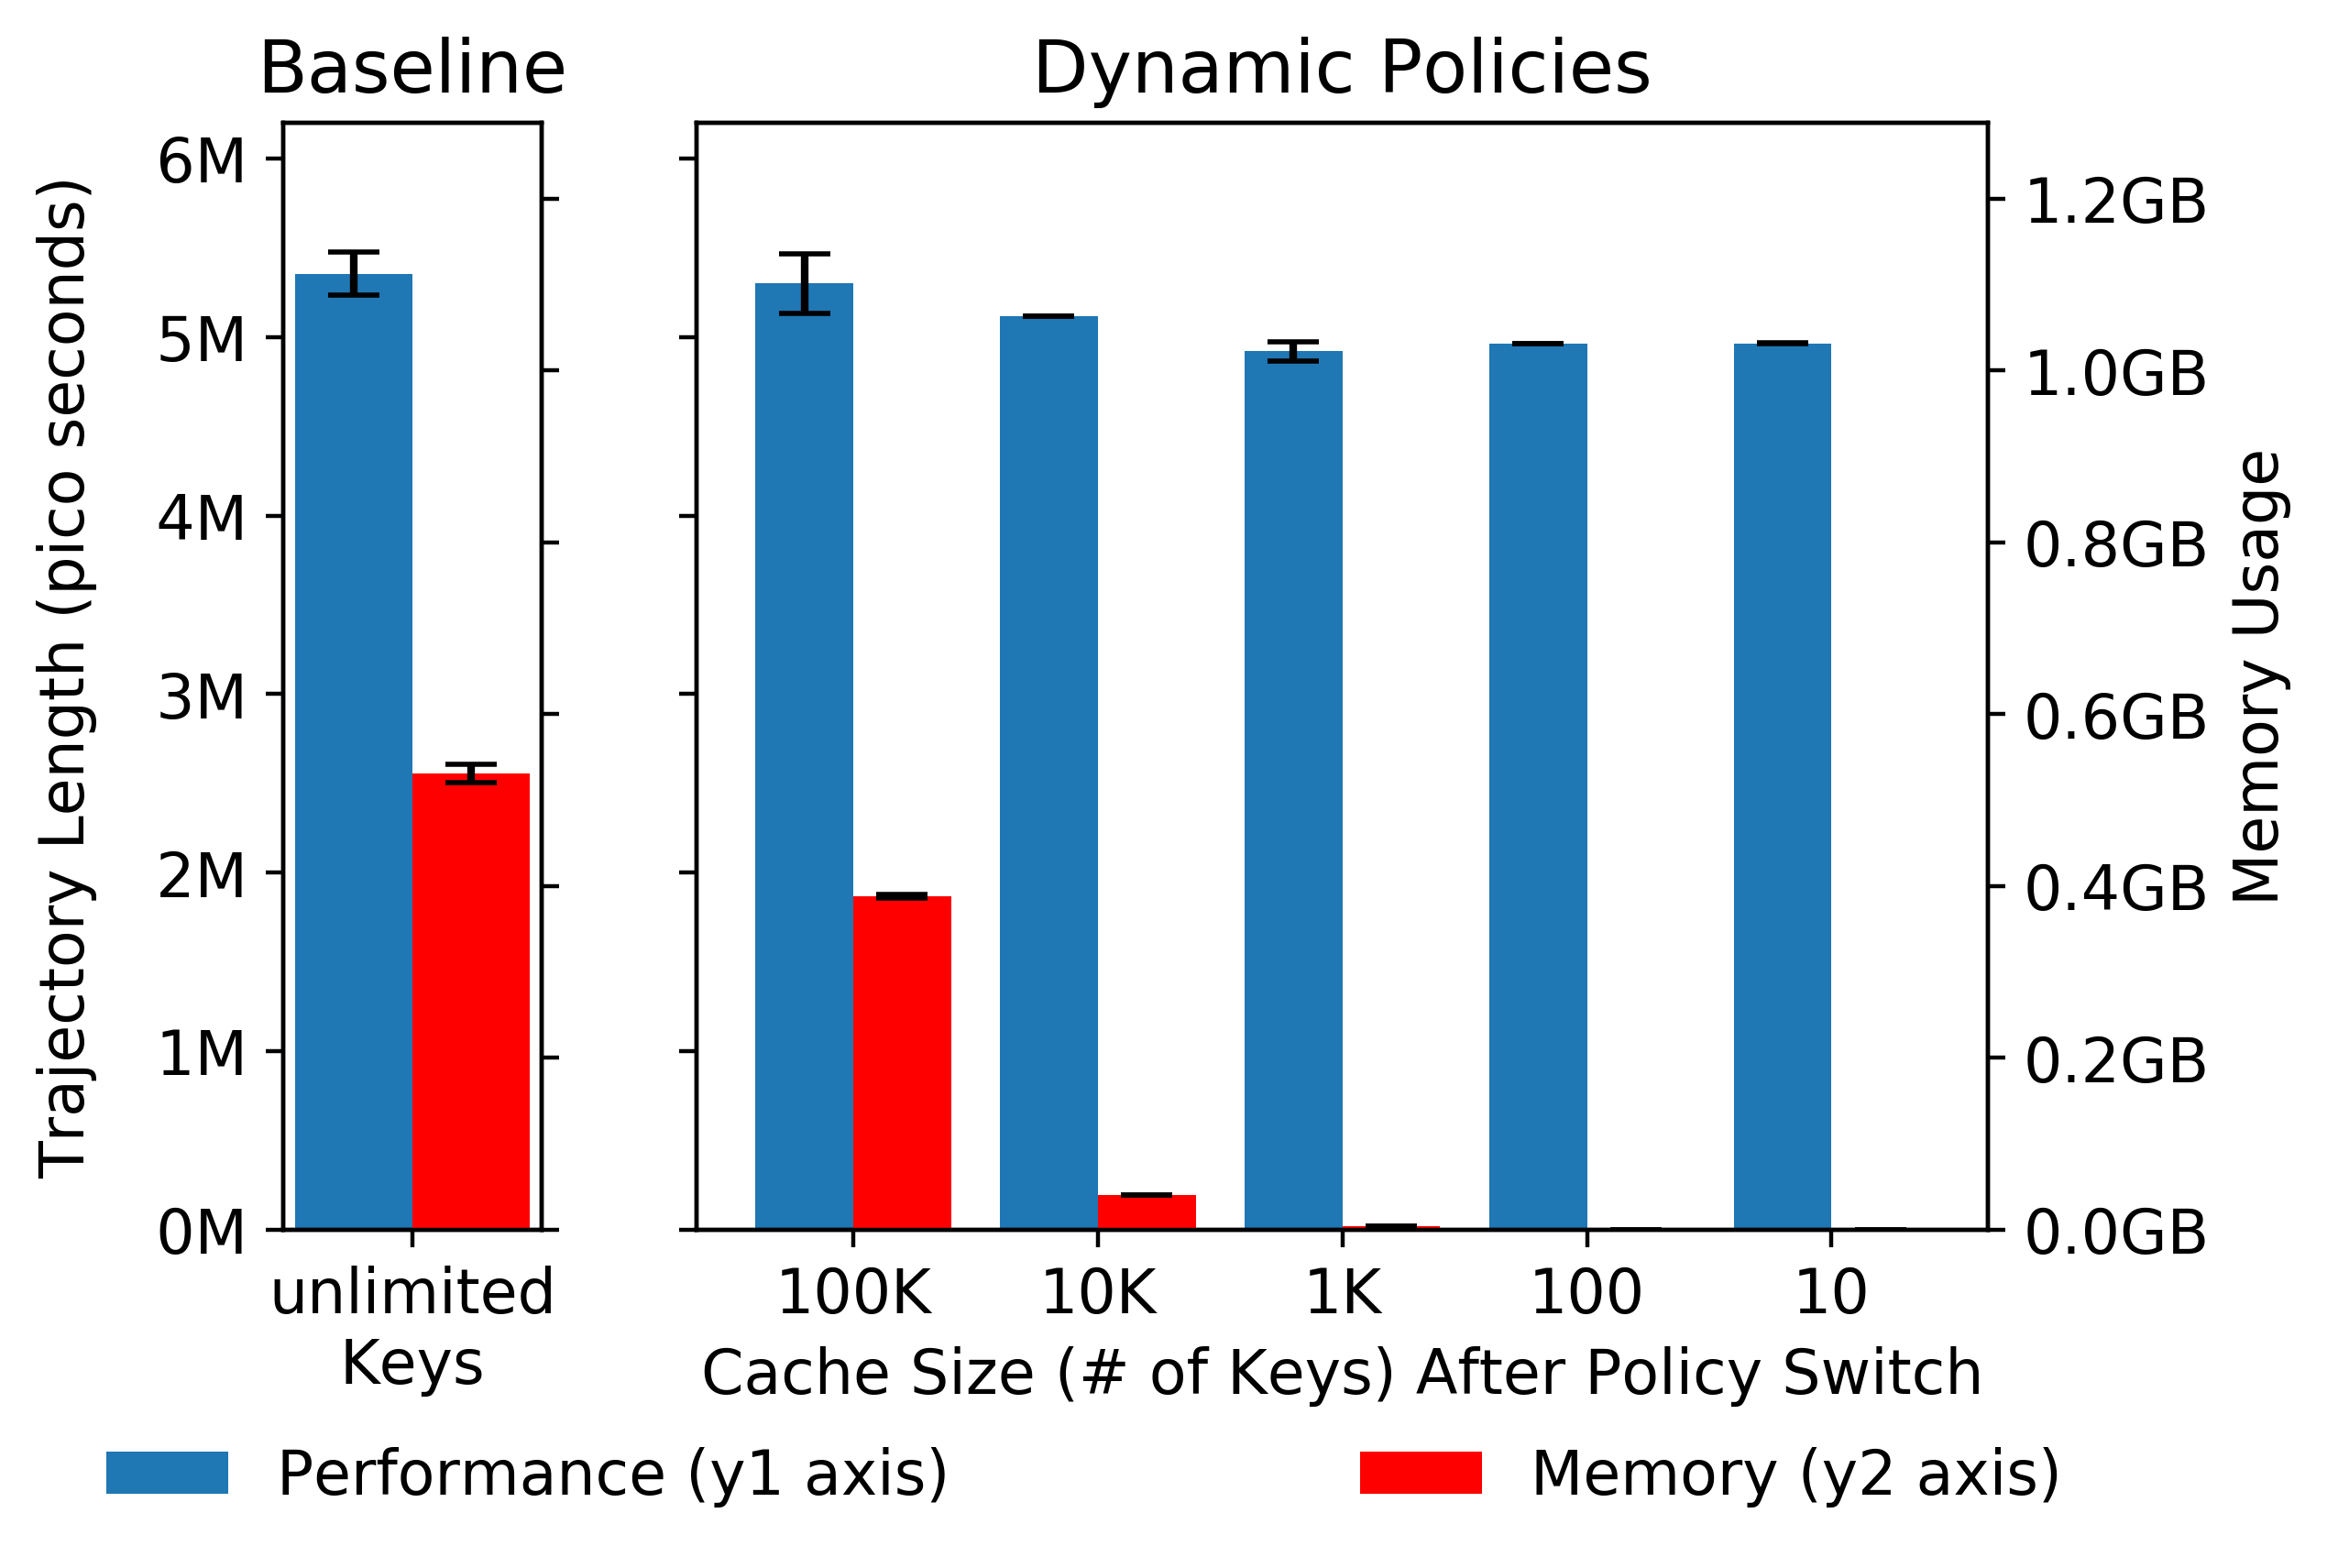
\includegraphics[height=4.5cm,width=0.4\textwidth]{figures/methodology-tradeoff-dynamic.png}\\
  \caption{The performance and resource utilization trade-off of using a
  dynamic load balancing policy that switches to a smaller cache after absorbing
  the initial burstiness of the workload. The sizes of these smaller caches are
  on the \(x\) axis.  \label{fig:methodology-tradeoff-dynamic}}
\end{figure}

Figure~\ref{fig:methodology-tradeoff-dynamic} shows the results of using the
Mantle API to program a dynamic load balancing policy into
ParSplice:

\begin{itemize}
  \item unlimited growth policy: cache increases on every write
  \item \(n\) key limit policy: cache constrained to \(n\) keys
\end{itemize}

We trigger the policy switch at 100K keys to absorb the flash crowd at the
beginning of the run. Once triggered, keys are evicted to bring the size of the
cache down to the threshold and the least recently used keys are evicted.
In that bar chart, the cache sizes are along the \(x\) axis.

% results: same level of performance can be achieved 
The dynamic policies show better performance than the single \(n\) key
policies. The performance and memory utilization for a 100K key cache size is
the same as the 100K bar in the middle graphs but the rest reduce the size of
the keyspace after the read flash crowd. This reduces read/write traffic on the
persistent database and lowers the number of stalls.  We see the worst
performance when the engine switches to the 10 key limit policy, which achieves
94\% of the performance while only using 40KB of memory. 

% caveats: it is calculating 90% of the trajectory, memory value reported is final
\subsubsection*{Caveats}

The results in Figure~\ref{fig:methodology-tradeoff-dynamic} are slightly
deceiving for three reason: (1) segments take longer to generate later in the
run, (2) the memory footprint is the value at the end of 2.5 hours, and (3)
this policy only works well for the 2.5 hour run.  For (1), the curving down of
the simulation vs. wall-clock time is shown in
Figure~\ref{fig:methodology-trajectory}; as the nanoparticle grows it takes
longer to generate segments so by the time we reach 2 hours, over 90\% of the
trajectory is already generated.  For (2), the memory footprint is around 0.4GB
until we reach 100K key threshold. In
Figures~\ref{fig:methodology-tradeoff}
and~\ref{fig:methodology-tradeoff-dynamic} we plot the final value. For (3),
Figure~\ref{fig:methodology-trajectory} shows that the cache fills up with 100K
keys at time 7200 seconds and its size is reduced to the size listed in the
legend.  The curves stay close to ``Unlimited" for up to an hour after the
cache is reduced but eventually flatten out as the persistent database gets
overloaded. 10K and 100K follow the ``Unlimited" curve the longest and are
sufficient policies for the 2.5 hour runs but anything longer would need a
different dynamic load balancing policy.

\begin{figure}[t]
  \noindent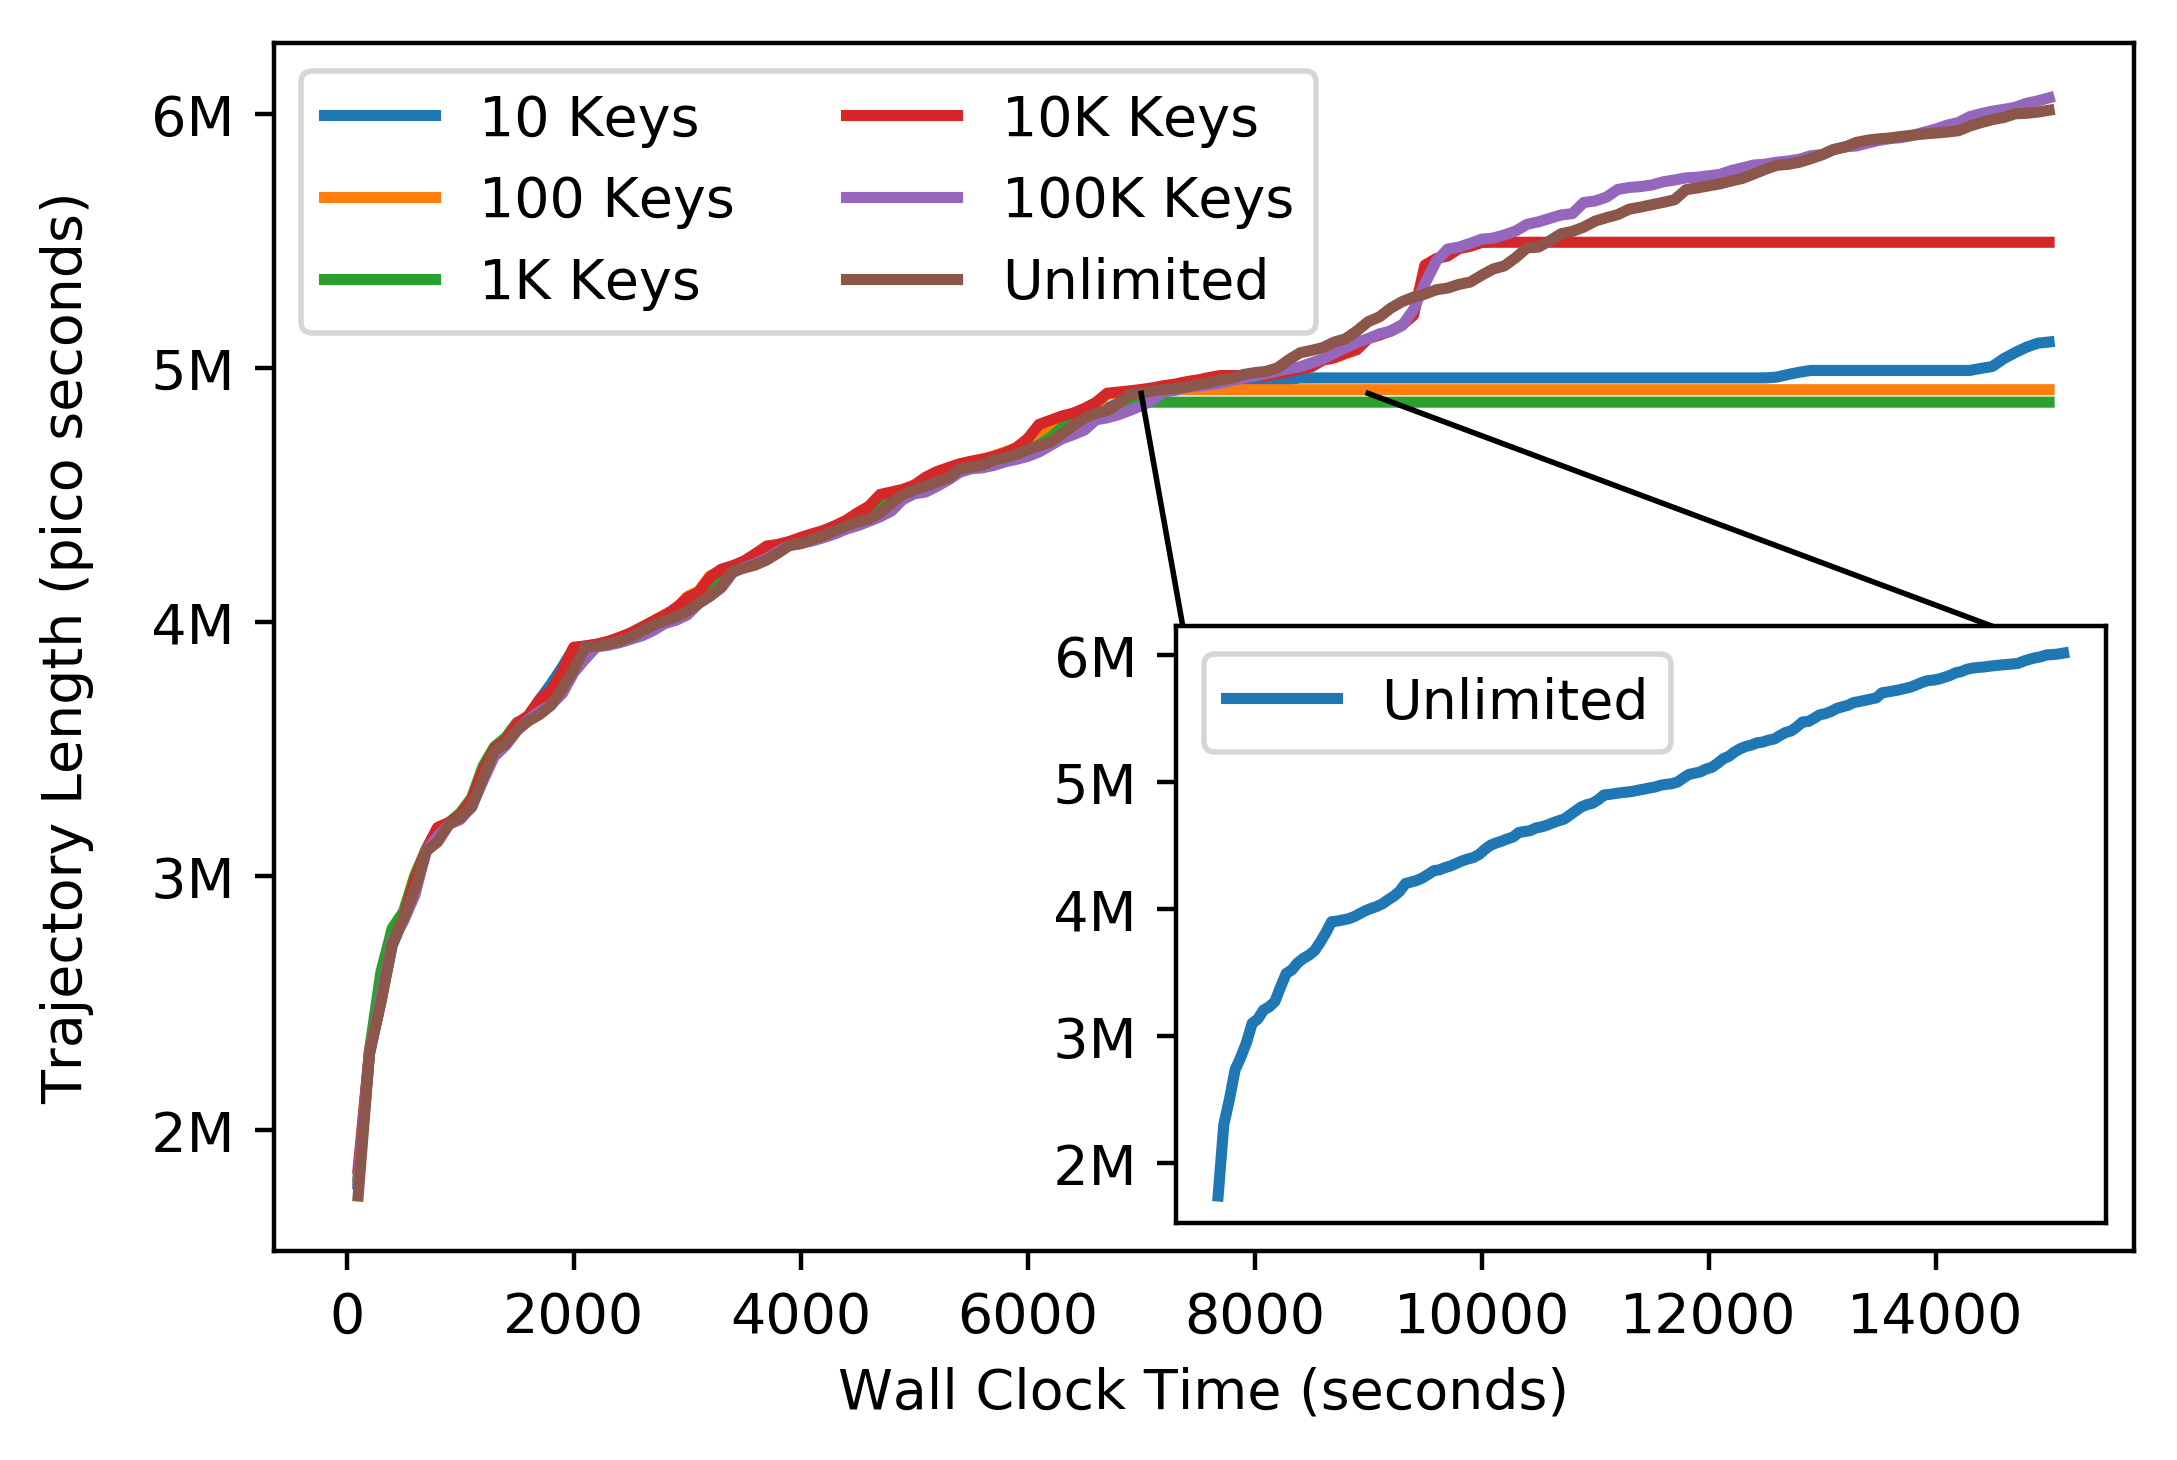
\includegraphics[height=4.5cm,width=0.4\textwidth]{figures/methodology-trajectory.png}\\
  \caption{The rate that the trajectory is computed decays over time (which is
  expected) but this skews the performance improvements in
  Figure~\ref{fig:methodology-tradeoff-dynamic}. Our dynamic policy works for 2.5
  hour jobs but not for 4 hour jobs.  \label{fig:methodology-trajectory}}
\end{figure}

% but the result is still valid
Despite these caveats, the result is still valid: we found a dynamic load
balancing policy that absorbs the cost of a high read throughput on a small
keyspace and reduces the memory pressure for a 2.5 hour run. Our experiments
show the effectiveness of the load balancing policy engine we integrated into
ParSplice, not that we were able to identify the best policy for all system
setups ({\it i.e.} different ParSplice parameters, number of worker tasks, and
job lengths).  To solve that problem, we need a way to identify what thresholds
we should use for different job permutations.


